\section{Problem Definition}
\begin{figure}
  \centering
  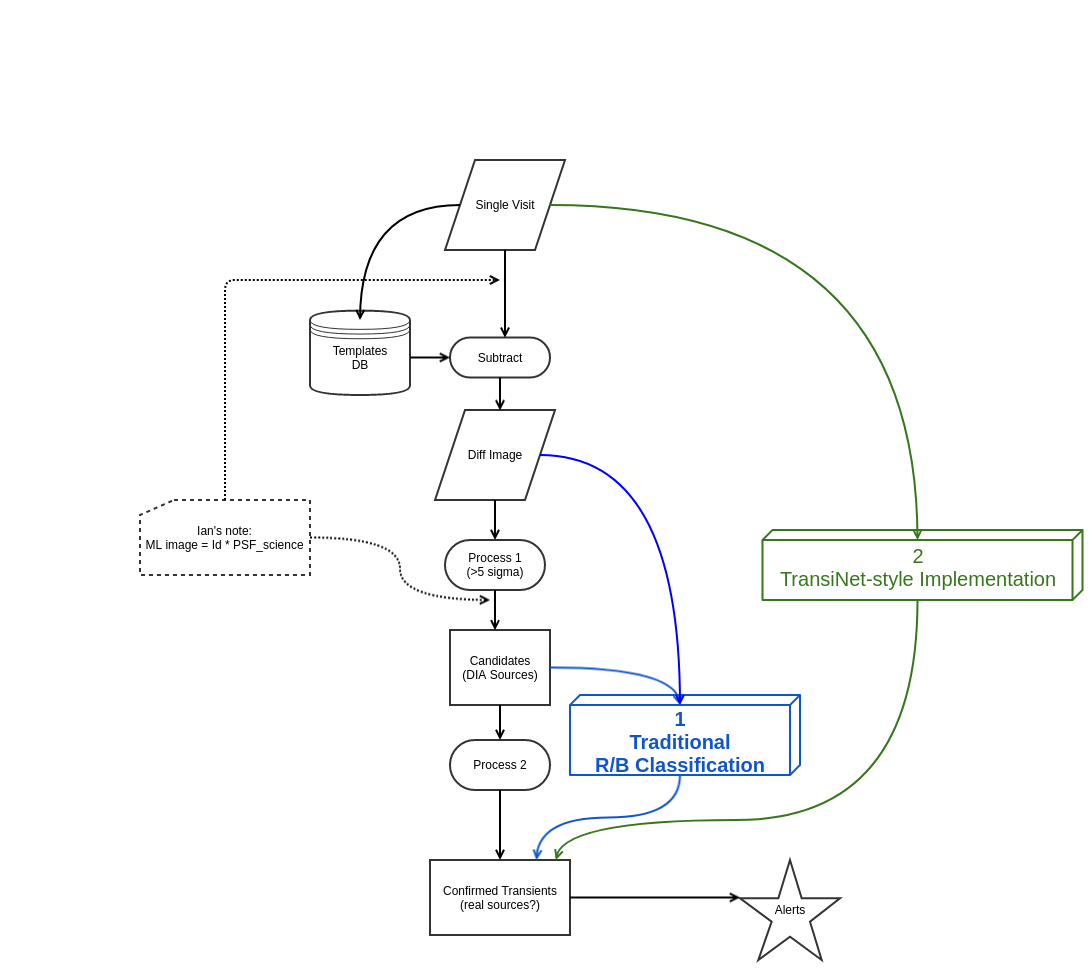
\includegraphics[width=1\textwidth]{material/diagram}
  \caption{Coarse illustration of information flow through the Alert Production (AP) pipeline. Paths in blue and green illustrate the ``traditional'' and ``modern'' approaches respectively.}
\end{figure}

% \section{Notes from the template}

% \subsection{How to handle LSST standard references?} 

% The papers should cite standard LSST references\footnote{See \url{https://github.com/lsst-pst/LSSTreferences}}, 
% where appropriate. For the usage, please see below.  These examples all use the ADS handle, unless they are 
% project docs then the use the project handle like LSE-17.

% All are on the lsst-texmf which you can get from \url{http://lsst-texmf.lsst.io}


% \subsubsection{LSST System and Science}

% The LSST system (brief overview of telescope, camera and data management subsystems),
% science drivers and science forecasts are described in:

% \begin{itemize}
% \item LSST Science Requirements Document: \cite{LPM-17}.
% \item LSST overview paper: \cite{2008arXiv0805.2366I}.
% \item LSST Science Book: \cite{abell2009lsst}.
% \end{itemize}
% %------------------------------------------------------------------------------


% \subsubsection{Simulations}

% The LSST simulations are described in a series of papers. Use of the LSST simulations should cite the LSST simulations overview paper \cite{2014SPIE.9150E..14C} and the specific simulation tools used:

% \begin{itemize}
% \item LSST Catalogs (CatSim): \cite{2014SPIE.9150E..14C}
% \item Feature-Based Scheduler: \cite{2018arXiv181004815N}
% \item Operations Simulator (OpSim): Scheduler \cite{2016SPIE.9910E..13D}, SOCS \cite{2016SPIE.9911E..25R}
% \item Metrics Analysis Framework (MAF): \cite{2014SPIE.9149E..0BJ}
% \item Image simulations (Phosim): \cite{2015ApJS..218...14P}
% \item Sky brightness model: \cite{2016SPIE.9910E..1AY}
% \item LSST Performance for NEO (or moving object) discovery: \cite{2018Icar..303..181J}
% \end{itemize}
% %------------------------------------------------------------------------------


% \subsubsection{Data Management}

% LSST data management system and the data products are described in:

% \begin{itemize}
%   \item The LSST Data Management System: \cite{2015arXiv151207914J}
%   \item Data Products Definition Document: \cite{LSE-163}
% \end{itemize}
%  %------------------------------------------------------------------------------


% \subsubsection{Camera}

% \begin{itemize}
%    \item Design and development of the LSST camera: \cite{2010SPIE.7735E..0JK}
% \end{itemize}
% %------------------------------------------------------------------------------


% \subsubsection{Telescope and Site}

% \begin{itemize}
%    \item Telescope and site overview and status in 2014:  \cite{2014SPIE.9145E..1AG}
% \end{itemize}
% %------------------------------------------------------------------------------

% \subsubsection{System Engineering}

% \begin{itemize}
%    \item LSST systems engineering: \cite{2014SPIE.9150E..0MC}
%    \item System verification and validation: \cite{2014SPIE.9150E..0NS}
% \end{itemize}
% %


